\par During stable LHC runs in Run~I and Run~II proton bunches collided at \SI{40}{\mega\hertz}; 
the current ATLAS data storage system however can only record events at about \SI{200}{\hertz}.
The ATLAS Trigger~\cite{PERF-2011-02} is responsible for selecting potentially interesting collisions
 and discarding the rest, reducing the \SI{40}{\mega\hertz} to about \SI{100}{\hertz}.
This reduction was achieved in 3  and 2 levels during Run~I and Run~II respectively.

\subsubsection{Level 1 }
\par Level 1 Trigger~\cite{1742-6596-396-1-012010} (L1) during Run~II is almost 
identical to that used in Run~I. In Run~I it reduced the \SI{40}{\mega\hertz} rate to about \SI{65}{\kilo\hertz}
while in Run~II it reduced it to \SI{100}{\kilo\hertz}.
The decision to accept or reject a bunch crossing is based on the multiplicity 
of physics objects ($e,\gamma,\mu,\tau,\met$ and jets) from that crossing with energies that pass 
any of the energy thresholds in a pre-defined set. The definitions of these physics objects is discussed in more 
detail in Chapter~\ref{obj}. To keep up with the \SI{40}{\mega\hertz} bunch crossing rate,
the maximum time to make the decision (latency) is kept \SI{2.5}{\micron}.
Signals from the EM and the hadronic calorimeters are used 
to construct $e,\gamma,\tau$ and jet candidates based on shower shape properties 
while patterns of hits from the muon spectrometer chambers are used to construct $\mu$ candidates and their \pT.
All these physics objects are assigned to a Bunch-Crossing Identification (BCID),  
which tags them to a specific proton bunch crossing. After all known physics 
objects are identified, \met\ is constructed as the remainder that enables the system to conserve 
transverse momentum. 

\par To keep up with the \SI{2.5}{\micron} latency, \acrshort{l1} has no access to full calorimeter granularity.
Rather, it uses groups of cells called Trigger Towers (TTs) of size $\eta\times\phi = 0.1\times0.1$. 
As described in Section~\ref{sec:calo} and as shown in Figure~\ref{fig:emCalSeg} the EM Cal 
comprises four layers of varying segmentation in $r$. The number of cells that make up a \acrshort{tt} 
is therefore dependent on the EM Cal layer. In Layer 2 one \acrshort{tt} comprises $4\times 4$ cells while in 
Layer 3 it comprises $2\times 4$ cells in $\eta\times\phi$. Since Layer 2 has the largest radiation length and 
contains most of the energy deposit, the feature extraction algorithm uses it as seed in searching for physics 
objects. The $e/\gamma$ algorithm first runs a sliding window to 
find a local maximum that comprises $2\times 2$ \acrshort{tt}s in $\eta\times\phi$. 
These $2\times 2$ tower regions shown in green in Figure~\ref{fig:TTalg} 
are called {\it clusters}. The algorithm then computes the horizontal and vertical sums of energy 
in this local maximum and labels the highest as the candidate energy for the cluster. 
The neighboring towers that sorround the cluster make up the Isolation Ring (IR), which is used to 
distinguish between shower profiles from different particles. The $\tau$ algorithm is 
similar to the $e/\gamma$ algorithm except that it allows showers to penetrate into the hadronic 
calorimeter because $\tau$s can decay to collimated clusters of hadrons.   
Showers detected in the hadronic calorimeter are 
labeled as jets. Since $\tau$ objects also leave showers in this region of the calorimeter, they are a special 
kind of jets that satisfy extra isolation requirements. Regardless, there is a dedicated algorithm for searching 
for jets. The procedure is similar to the $e/\gamma$ algorithm, 
but it instead uses $4\times 4$ \acrshort{tt} windows called {\it jet elements} 
(groups of \acrshort{tt}s $0.2\times 0.2$ in $\eta\times\phi$).   

\begin{figure}[!h]
\centering
   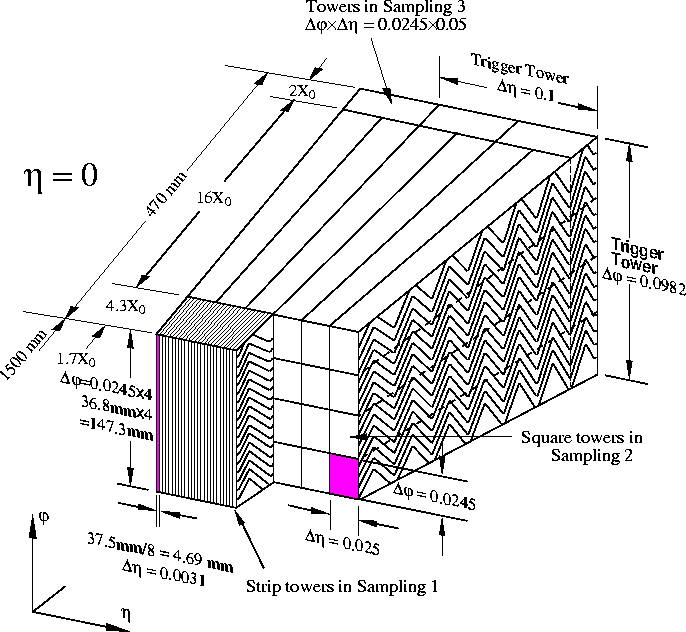
\includegraphics[width=0.8\textwidth]{figures/emCalSeg.png}
	\caption{Schematic diagram of showing cell segmentation in the EM Cal, across multiple layers}
	\label{fig:emCalSeg}
\end{figure}

\begin{figure}[!h]
\centering
   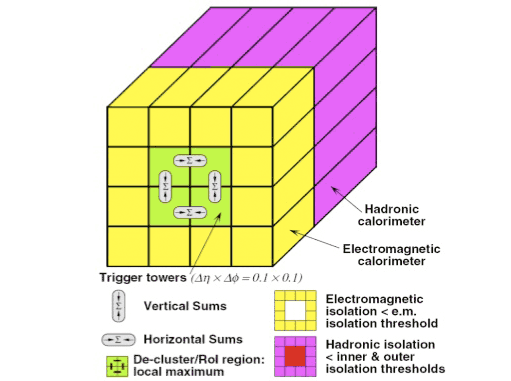
\includegraphics[width=0.8\textwidth]{figures/TTalg.png}
	\caption{Illustration of the search algorithm for electrons and photons in the EM Cal}
	\label{fig:TTalg}
\end{figure}

\par With a \SI{1.5}{\ns} time resolution, \acrshort{rpc}s and \acrshort{tgc}s in the Muon Spectrometer 
offer muon hits in all three dimensions in the barrel and end-cap regions 
respectively. The goal of the muon trigger is to identify muons originating 
from the interaction point. As discussed in Section~\ref{sec:muonSpec} \acrshort{rpc}s are 
arranged in three layers. Just like in the calorimeters the second \acrshort{rpc} layer is used as seed 
in identifying a muon track. In this case a \acrshort{tt} is of size $\Delta\phi\times\Delta\eta = 0.2\times0.2$.
 If a hit is found in the second layer, a {\it coincidence 
window} in relation with the hit is defined in the first and third layers based on the 
line connecting the hit and the interaction point. Hits are then searched in the coincidence 
window in the first and third layer. If more than one hit is found in the first 
and third layers, multiple hit combinations are combined in parallel and one 
with the highest acceptance probability of \pT~greater than a given threshold 
is picked. A similar algorithm is employed in the end-caps where TGCs handle the 
relatively higher muon rates. 

\par For events that pass \acrshort{l1} coordinates of the detector where physics 
objects that triggered \acrshort{l1}, their \pT\ and the \acrshort{bcid} are saved 
in buffers and handed over to upper levels of the trigger. This information is called 
a Region of Interest (RoI). 

\subsubsection{Example Shower Profile Classification}
\label{sec:bnl}
\par As discussed above, algorithms used at \acrshort{l1} are designed to 
distinguish between hadronic showers and EM showers. The EM showers in most 
cases are initiated by electrons and photons ($e/\gamma)$.  
Due to the limited calorimeter granularity available at \acrshort{l1}, it is difficult to distinguish 
some hadronic showers from $e/\gamma$ showers. A case in point is a \pizero\  
versus an electron. With a lifetime 
of about ~\SI{8e-17}{\s} the \pizero\ immediately decays to a pair of photons when it 
interacts with the calorimeter absorber material. These two photons each initiate an 
EM shower that is hardly distinguishable using the \acrshort{l1} algorithms in the preceding section. 

\par The strategy used to distinguish between \pizero\ and electron showers relies heavily on 
resolving the two photon showers contained within the \pizero\ shower. Simulation studies 
have shown that \acrshort{tt}s are too coarse to resolve these two photon showers, so such a strategy is 
employed at Level 2 (see Section~\ref{sec:hlt}). As the instantaneous luminosity of the LHC is expected 
to more than double by 2022, the trigger is expected to handle more input data. One way to ensure 
that trigger rates are kept constant is to upgrade \acrshort{l1} such that it becomes capable of perfoming 
some of the tasks that would otherwise be left for \acrshort{l2}. One of such tasks is the 
classification of $\pizero/e$ showers.      

\par An improvement in granularity from \acrshort{tt}s at \acrshort{l1} 
was explored as a potential setup to separate \pizero~showers 
from electron showers. This upgrade would constitute upgrading from \acrshort{tt}s to {\it supercells}, 
where a supercell is a group of calorimeter cells that span a $0.025\times0.1$ region in $\eta,\phi$. 
More precisely, 1 supercell corresponds to 1 cell in the EM Cal presampler, 8 in Layer 1 and 4 in Layer 2. 
In Layer 3 the cell granularity in $\eta$ is coarser than a single supercell, so no segmentation is required. 
The objective of this study was to determine the feasibility of rejecting more than 
50\% \pizero\ showers while retaining at least 95\% of electron showers using supercell granularity. 
This amounts to deriving variables that quantify shower shapes in the lateral and longitudinal 
planes and distinguishing between shapes due to \pizero to those due to electrons.  

\par The procedure for obtaining simulation data samples is the
following : Single, isolated electrons or \pizero s were generated
with a predefined energy and direction in ($\eta, \phi$) in the EM
Cal. For simplicity the chosen direction ($\eta=0.4125, \phi=0.1125$)
 is the center of a cell. Geant4~\cite{Agostinelli2003250} was used to
simulate the EM Cal. The output of this simulation was digitized and
subsequently reconstructed. Separate samples were also made in which electrons and
\pizero s were generated over a range in $\eta$ covering the width
of a cell in Layer 2 ($\Delta\eta = 0.025$), which is also the width of
a supercell. These samples are referred to as {\it
scanned $\eta$} samples. Contrastingly, samples generated in the standard manner  
 are called {\it fixed $\eta$} samples. By default, simulated particles were 
generated from the interaction point. A simplistic model of the generation point 
be described by a $\delta-$function at $z=0$ while a more realistic one with a Gaussian distribution with RMS
$\approx$ \SI{5}{\cm}. Smearing the interaction point with a known RMS is 
referred to in this thesis as {\it vertex smearing}.

\par Figure~\ref{fig:bnlRes} shows a comparison of electron and \pizero\ 
showers using several variables that exploit the difference in their 
longitudinal and lateral profiles. For longitudinal comparisons the fraction 
of energy deposited in a layer and cluster {\it cl} is used. It is  
quantified by $\rho_{\textrm{layer}}$ where 

\begin{equation}
\rho_{\textrm{layer}} = \frac{\sum_{\textrm{c}\in\textrm{cl},\textrm{c}\in\textrm{layer}}\textrm{(E}_{\textrm{c}}\textrm{)}}{\textrm{E}_{\textrm{cl}}}.
\end{equation}

$\rho_{\textrm{layer}}$ can be used to classify electrons and \pizero s of low \pT\ but it 
loses its robustness for those of high \pT. The same can be said of $\rho_{\textrm{comp}}=\frac{\rho_{1}}{\rho_{2}}$, 
which is a comparison between  $\rho_{\textrm{layer}}$ from Layer 1 and Layer 2. To study lateral profiles 
the ratio of the energy deposited in the supercell with the highest energy deposited (colloquially 
referred to as the {\it hottest} supercell), to the sum of that energy and the 
energy deposited in the two neighboring supercells in $\eta$ is used. This ratio is quantified as 

\begin{equation}
\textrm{R}_{\eta}^{(1)} = \frac{\textrm{E}_{0}}{\textrm{E}_{+1} + \textrm{E}_{0} + \textrm{E}_{-1}},
\end{equation}  

where $\textrm{E}_{0}$ is the energy deposited in the hottest supercell, $\textrm{E}_{1}$ in the 
supercell to the right of the hottest supercell and $\textrm{E}_{-1}$ to the left of the 
hottest supercell. $\textrm{R}_{\eta}^{(1)}$ performs superbly for low \pT electrons and \pizero s.
For high \pT\ it becomes less robust but can still classify electrons and \pizero s with high 
accuracy. Figure~\ref{fig:bnlRes} shows that for 20~\GeV\ \pizero s and electrons more than 50\% 
\pizero s are rejected while less than 5\% electrons are accepted. In the more realistic case 
where vertex smearing is turned on and the $\eta$ position is scanned however, $\textrm{R}_{\eta}^{(1)}$ 
loses its robustness.   

\par These results show that even with supercell granularity at L1, separation between electrons 
and \pizero s is not a trivial subject. More studies on this subject will have to be done 
during the long LHC shutdown that starts in 2018 to meet the higher trigger rates that ATLAS has 
to face afterwards. 

\begin{figure}[!h]
   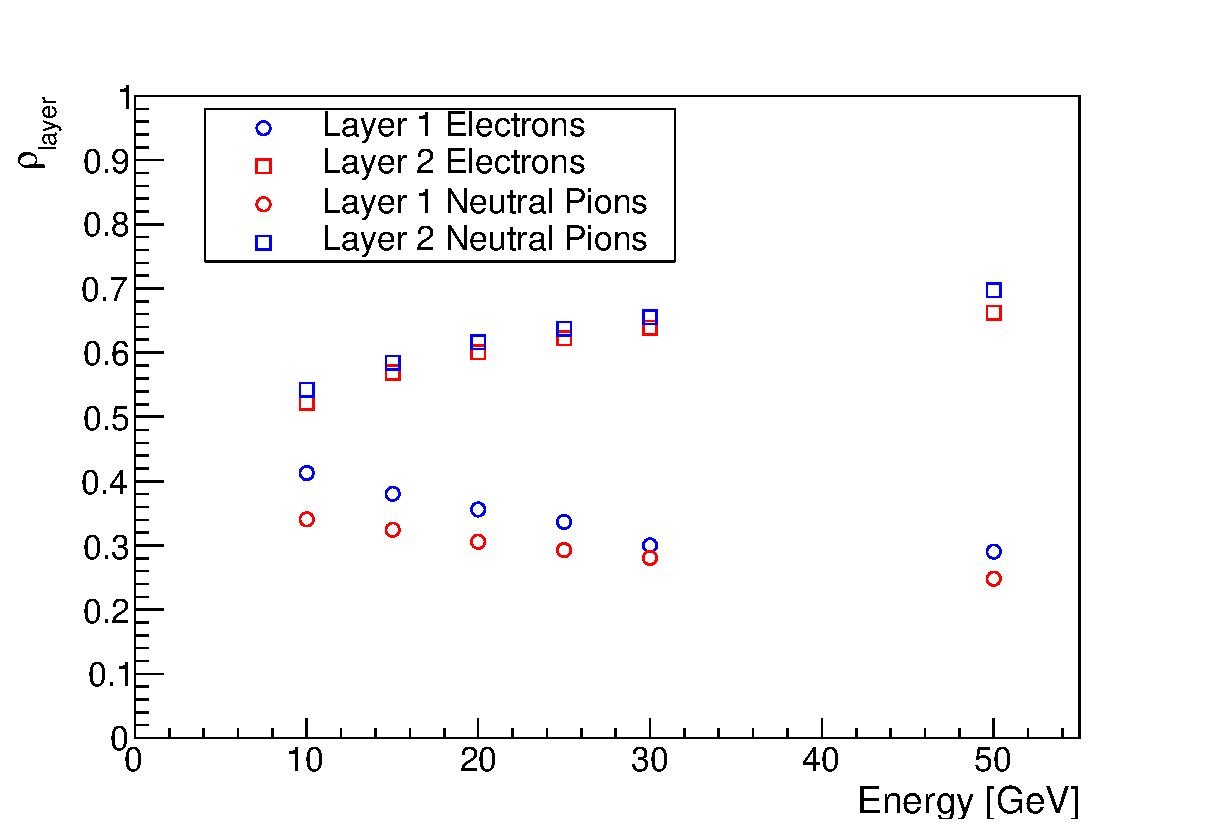
\includegraphics[width=0.5\textwidth]{figures/rhoLayer12.eps}
   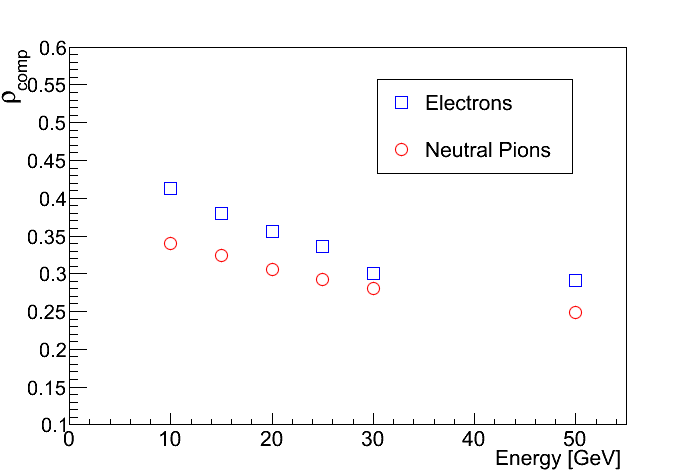
\includegraphics[width=0.5\textwidth]{figures/rhoComp.png}\\
   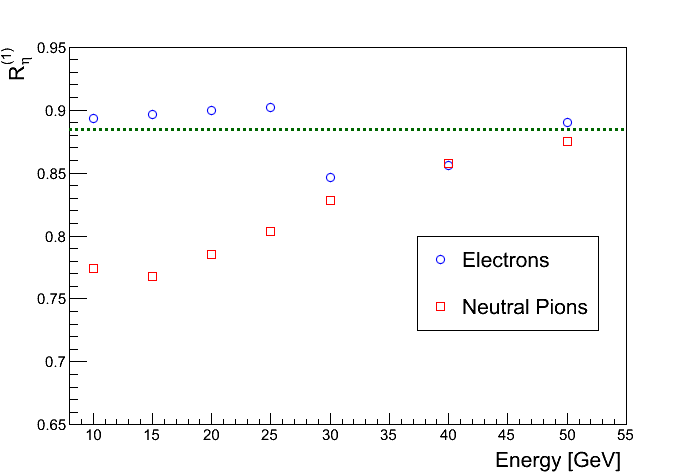
\includegraphics[width=0.5\textwidth]{figures/retaonelrCloseup.png}
   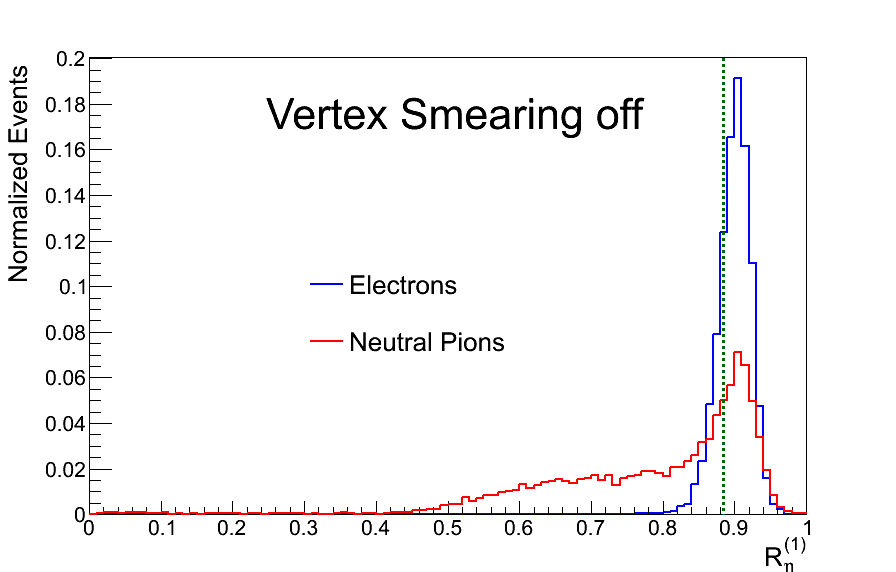
\includegraphics[width=0.5\textwidth]{figures/retaonelrTwenty.png}\\
  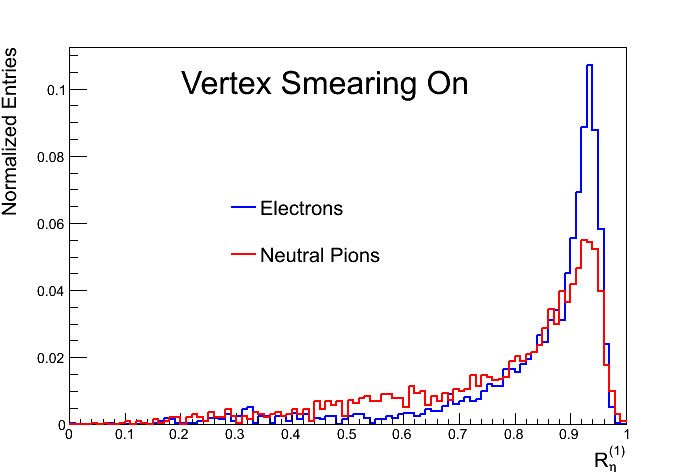
\includegraphics[width=0.5\linewidth]{figures/RetaVx.png}%
  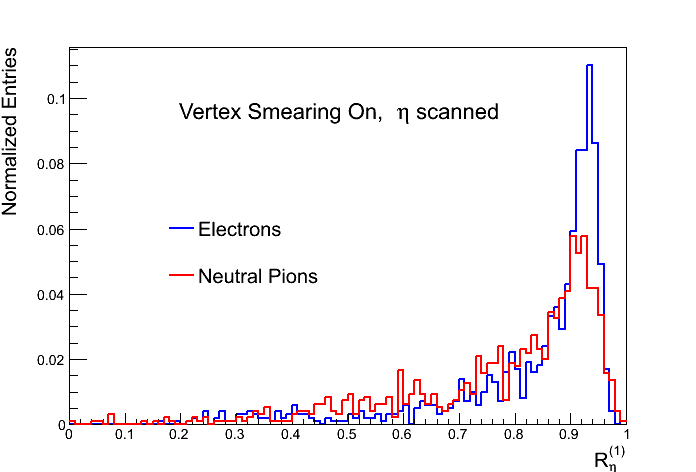
\includegraphics[width=0.5\linewidth]{figures/Scan.png}%
	\caption{Distributions of variables used to separate electrons and \pizero s. 
[Top Left] $\rho_{\textrm{layer}}$ for Layer 1 and Layer 2. [Top Right] $\rho_{\textrm{comp}}$ for 
Layer 1 and Layer 2. [Middle Left] $\textrm{R}_{\eta}^{(1)}$ for \pizero s and electrons across 
several energies. [Middle Right]  $\textrm{R}_{\eta}^{(1)}$ for 20~\GeV\ electrons and \pizero s.
[Bottom Left] $\textrm{R}_{\eta}^{(1)}$ with vertex smearing on. [Bottom Right] $\textrm{R}_{\eta}^{(1)}$
 with vertex smearing turned on and $\eta$ scanned across a 0.025 range}
	\label{fig:bnlRes}
\end{figure}

\subsubsection{High Level Trigger and Data Acquisition}
\label{sec:hlt}
\par The High Level Trigger~\cite{5321918} (HLT) is responsible for reducing the rate from \SI{100}{\kilo\hertz} 
to about \SI{100}{\hertz}. During Run~I it comprised two separate levels : Level 2~\cite{dosanjos:in2p3-00148815} (L2)
 that reduced the rate to \SI{1}{\kilo\hertz} and the Event Filter~\cite{Negri2007} (EF) that reduced 
it to \SI{100}{\hertz}. During Run~II a lot of components in L2 were combined with the EF.
 Data management is handled by a separate system 
called Data Acquisition~\cite{5321758} (DAQ). So combined, the HLT and DAQ are referred to as TDAQ. 

\par To minimize latency, input to the \acrshort{hlt} is a set of \acrshort{roi}s from \acrshort{l1} 
whose associated data is just a few percentage of the raw data. The rest of the raw data 
are kept in buffers known as Readout Buffers (ROBs) and are extracted upon request using the
Readout System (ROS) by the Data Collection Manager (DCM). For \acrshort{l2}, \acrshort{roi}s are assembled by a 
Region Of Interest Builder (RoIB) and passed over to a farm of Linux PCs.
Here five L2 Supervisors (L2SVs) schedule and assign events to nodes on the Linux farm. 
L2 Processing Units (L2PUs) run event selection algorithms on the \acrshort{roi} while taking 
advantage of the full calorimeter granularity and requesting more data 
from \acrshort{rob}s when necessary. These selection algorithms take a wholistic approach by making decisions 
based on \acrshort{roi}s from a combination of detector components. For example, information from both the \acrshort{id}
and the Muon Spectrometer is used to identify muons and their \pT.  
Ultimately, \acrshort{l2pu}s report their decisions back to \acrshort{l2sv}s, which pass the decisions and logs to L2 Result Handlers (L2RH).

\par During Run~I, upon \acrshort{l2} acceptance event raw data was passed to a
separate farm of Linux PCs that ran \acrshort{ef} off-line event selection algorithms. 
These algorithms were similar to \acrshort{l2} 
algorithms but included the latest calibrations and alignment information. During Run~II a series of upgrades 
were executed that merged \acrshort{l2} and \acrshort{ef} Linux PC farms, where each \acrshort{hlt} node accepts
the \acrshort{roi}s through the \acrshort{roib}, makes a decision, 
builds the event and executes the \acrshort{ef} algorithms. In this setup new but fewer components 
are introduced: the High Level Trigger Supervisor (HLTSV), the High Level Trigger Processing Unit
 (HLTPU), and the \acrshort{dcm}. 
A component of the \acrshort{hltsv} replaces the \acrshort{l2sv}. Only one \acrshort{hltsv}
is needed to handle a pair of inputs, compared with 5 \acrshort{l2sv}s in Run~I. 
Additionally, the \acrshort{hltsv} is responsible for grouping decisions from the \acrshort{hltpu}s 
and sending them to \acrshort{ros} PCs to either clear or keep event fragments. The \acrshort{hltpu}s assumme the 
role similar to \acrshort{l2pu}s and the Event Filter Processing Units (\acrshort{efpu}s).
Each \acrshort{hltpu} is accompanied by a couple of \acrshort{dcm}s,
 which serve as media for collecting fragments from the \acrshort{hltsv}.  

\par A schematic of the Run~I setup is shown in Figure~\ref{trig_cur}. In this setup all components are run by
 applications on several PCs. The applications are configured and controlled by a 
common software framework~\cite{Barczyk:2003ya} referred to in this thesis at in 
the format {\it tdaq 05-xx-yy}, where {\it xx} and {\it yy} are release tags.
 The structure and settings of the system is specified in a set 
of XML files, which form a configuration database. Application configurations are grouped 
into {\it segments} that make up a {\it partition} when grouped together.
 The main configuration used at Point 1 
is called the {\it \acrshort{atlas} partition}. It is possible to create individual partitions 
parallel to the \acrshort{atlas}  partition for testing purposes, where 
network connections are handled by a common partition called the {\it initial} partition.

\begin{figure}[!h]
\centering
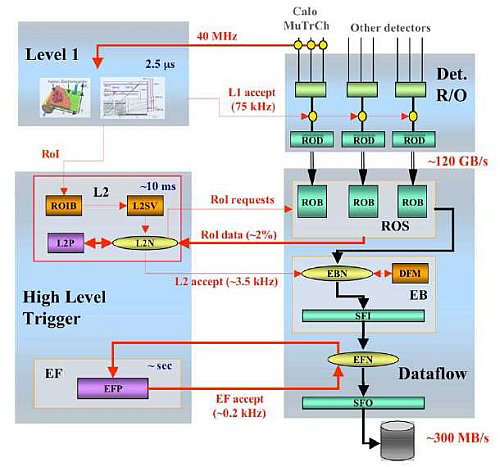
\includegraphics[width=0.8\linewidth]{figures/current_trig}
\caption{A schematic of the Run~I \acrshort{atlas} \acrshort{tdaq}. Data flow is depicted by black arrows and message flow by red. The \acrshort{l2} and the \acrshort{ef} run separate sets of algorithms on the data. Applications running in this system are configured under segments that make up a partition}
\label{trig_cur}
\end{figure}

\par There are three main reasons the Run~II trigger performs more efficiently than 
the Run~I trigger. First, the \acrshort{l2} and the \acrshort{ef} share a large fraction of code.
 Merging these two components reduces code duplication and optimizes resource usage. 
Second, \acrshort{roi} data are retrived twice Run~I while in Run~II data are retrieved once.
Third, the whole Run~II system has fewer components and is therefore easier to configure and optimize.
Section~\ref{sec:anlL2} discusses a study that was influential testing the feasibility of merging 
\acrshort{l2} with \acrshort{ef} to form the \acrshort{hlt}.

\subsubsection{Feasibility studies on HLT upgrade -- RoIB Evaluation Tests}
\label{sec:anlL2}

\par Argonne National Laboratory~\cite{anl} (ANL) hosts a farm of 13 Linux PCs that is a prototype 
of the farm at Point 1. This section discusses tests done on the RoIB using 
the \acrshort{anl} test stand. The goal was to determine if there is a configuration with 
which the RoIB can process events at \SI{100}{\kilo\hertz}. 

\par Special cards installed on the \acrshort{anl} PCs emulate elements of the 
Trigger and Data Acquisition (TDAQ) system. Two quad s-link transmitter (\acrshort{quest}) 
cards are used to supply \acrshort{l1} event fragments to the \acrshort{roib} via a VME crate with
 a VME Single Board Controller (VMESBC) that houses custom VME cards that combine \acrshort{l1} fragments. 
A Four Input Links for Atlas Readout (\acrshort{f}) card receives data fragments from the \acrshort{roib} 
and transmits it via a highly integrated PCIx interface to the \acrshort{hltsv}. A Two Input Links for 
Atlas (\acrshort{t}) card functions just as a \acrshort{f} card but with two less inputs and a PCIe interface.
Figure~\ref{filar} shows a chartflow of how the data fragments flow 
in a partition on this test bed : A \acrshort{quest} card reads data from simple text files and transmits 
the fragments to the \acrshort{roib}. After being processed by the \acrshort{roib} the fragments are 
relayed to the \acrshort{hltsv} via a \acrshort{f} or a \acrshort{t} card (tests were done with 
both cards and the rates were assessed independently). The \acrshort{hltsv} then assigns fragments 
to HLTPUs and also relays them to the \acrshort{ros}. Since these components of data-flow are 
located on multiple PCs, multiple optical cables facilitate inter-PC connection. 

\begin{figure}[!h]
\centering
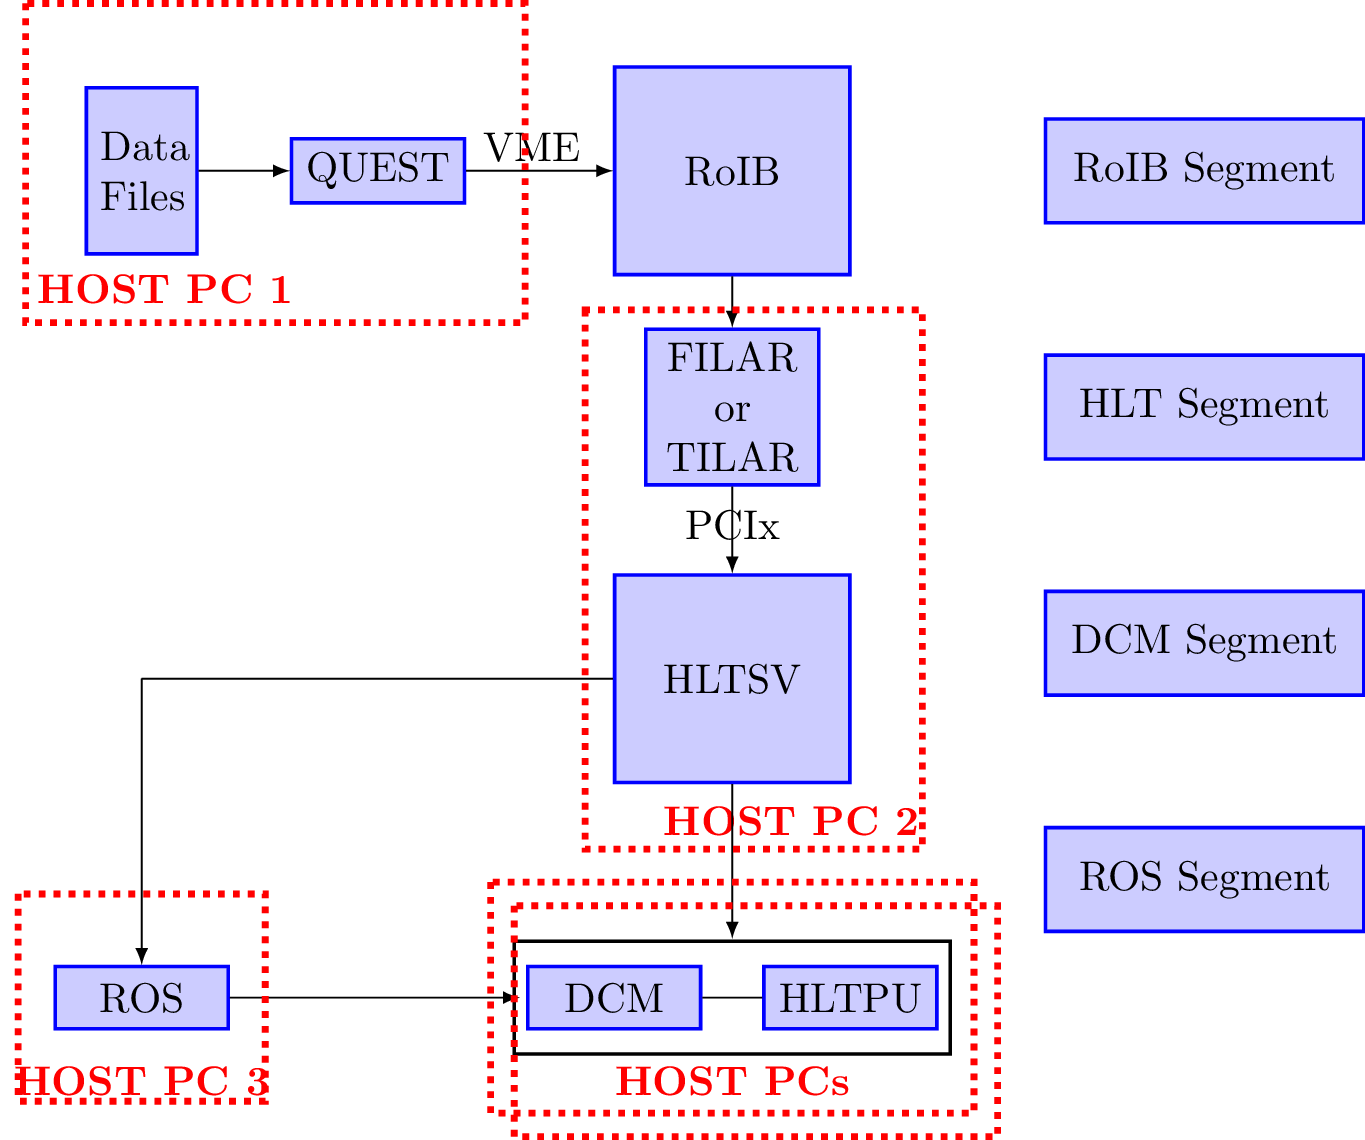
\includegraphics[width=0.8\linewidth]{figures/filar.png}
\caption{A flow-chart showing data flow in a partition at \acrshort{anl}'s test bed}
\label{filar}
\end{figure}

\par Table~\ref{pc} shows the PC specifications on the test bed and the special cards installed on 
those PCs. The PCs are identified as {\it ustb*}, where * is an integer in $[0,21]$ 
and ustb stands for `US Test Bed'.\footnote{Not all integers in \{0,21\} are used, because there are only 13 PCs} 
Since ustb16 hosts the \acrshort{f} card, the \acrshort{hltsv} application must run on ustb16. ustb3, ustb4
 and ustb10 are called {\it blade} PCs because they are single board ATCA computers that do not have 
PCIe or PCIx slots for \acrshort{f} or \acrshort{t} cards.  

\begin{table}[!h]
\begin{center}
\begin{tabular}{c|c|c|c|c|c|c|c|c|c|c}
Cards &PC&\multicolumn{2}{|c|}{Architecture} &\multicolumn{2}{|c|}{CPUs} &Cores &\multicolumn{2}{|c|}{HT} &Cache &Memory \\
      &  &32 Bits & 64 Bits &1 &2 & & Yes & No & [MB] & [MB] \\
\hline\hline
\acrshort{f} &ustb16 &\checkmark &  &\checkmark &  & 4 & &\checkmark & 6.1 & 4 012 \\
\hline
\multirow{2}{*}{\acrshort{quest}}& ustb14 &\checkmark & &\checkmark & & 4 & &\checkmark & 6.1 & 4 012 \\ 
& ustb21 &\checkmark & & &\checkmark & 8 & &\checkmark & 6.1 & 4 018 \\ 
\hline
\multirow{2}{*}{\acrshort{t}}& ustb0 &\checkmark & &\checkmark & & 4 & &\checkmark & 6.1 & 4 012 \\ 
& ustb11 &\checkmark & & &\checkmark & 8 & &\checkmark & 6.1 & 4 018 \\ 
\hline
\acrshort{robinnp} &ustb12 & &\checkmark & &\checkmark & 8 & &\checkmark & 6.1 & 3 921 \\
\hline
VMESBC &ustb7 &\checkmark &  &\checkmark &  & 1 & &\checkmark & 0.5 & 511 \\
\hline
 &ustb1 & &\checkmark  & &\checkmark & 8 &\checkmark & & 8.2 & 12 183 \\
 &ustb3 & &\checkmark  & &\checkmark & 8 &\checkmark & & 8.2 & 3 910 \\
 &ustb4 & &\checkmark  & &\checkmark & 8 &\checkmark & & 8.2 & 3 910 \\
 &ustb10 & &\checkmark  & &\checkmark & 12 &\checkmark & & 12.3 & 12 187 \\
 &ustb13 & &\checkmark  &\checkmark & & 4 & &\checkmark & 6.1 & 3 920 \\
 &ustb20 & &\checkmark  & &\checkmark & 8 & &\checkmark & 6.1 & 4 019 
\end{tabular}
\end{center}
\caption{Linux run PCs on the \acrshort{anl} Test Bed. They have diversely varying CPU strength 
and hardware structure, so some custom-made cards can only be installed on specific computers.
 {\it HT} stands for hyperthreading. The cores are the total number of cores in all the 
physical CPUs. \acrshort{f} and \acrshort{t} cards transmit data fragments from the \acrshort{roib} 
to the \acrshort{hltsv}. The \acrshort{quest} cards supplies data fragments to the \acrshort{roib}. 
Although ustb1, ustb3 and ustb10 are the most powerful, none can host any custom cards because they have a very thin structure.}
\label{pc}
\end{table}

\par There are three potential bottlenecks to the \acrshort{roib}/\acrshort{hltsv} rate.
 First is the link from the \acrshort{roib} to the \acrshort{f} card. Second is the PCIx connection from the
 \acrshort{f} card to the \acrshort{hltsv} and third is the CPU memory on 
which the \acrshort{hltsv} runs. It was shown at Point 1 that the maximum rate of transferring fragments 
from the \acrshort{roib} to the \acrshort{f} cards using one link is around \SI{60}{\kilo\hertz}. 
Using two optical fibres for the link would therefore achieve a \SI{100}{\kilo\hertz} 
rate of fragment transfer. This leaves two bottlenecks in the system, where the CPU bottleneck is very dominant.   
Just like in Run~I, the data flow in the Run~II \acrshort{daq} uses 
the {\it pull} architecture, as opposed to the {\it push} architecture. In the 
pull architecture when the HLTPU is done processing event fragments it sends a 
message to the \acrshort{hltsv}, which requests a set of fragments from the \acrshort{roib}.
 In tdaq 05-02-00, the \acrshort{f} card is limited by a single buffer whereas in tdaq 05-03-00
 the buffer size is increased to 100. Such a large buffer size causes problems with the 
driver -- version 05-03-00 of TDAQ that limits 
the \acrshort{f} card buffer size to 16 was used in these studies. The 100-buffer 
and 16-buffer versions are referred to as A and B respectively. 

 \par Table~\ref{parameters} shows some of the parameters that can be configured to 
optimize the \acrshort{hltsv} rate when running the \acrshort{roib}.
The \gls{dcmtest} is the application that handles \acrshort{dcm} functionalities. 
The NumberOfCores is the number of cores on which \acrshort{dcm}s run on. It is the same as 
the number of \acrshort{dcm}s in the system. L2ProcessingTime is the time it takes to run the 
\acrshort{l2} algorithms within HLTPUs. The EventBuildingTime is the time is 
takes to build the event if it is accepted by the \acrshort{l2} algorithms. 
The \gls{hltsvapp} is the application that runs the \acrshort{hltsv}. 
The NumberOfAssignedThreads are the core threads assigned to the \acrshort{hltsv}.

\begin{table}[!h]
\begin{center}
\begin{tabular}{c|c}
Application & Parameter \\
\hline\hline
HLTSV\_DCMTest & \gls{noc} \\
	& \gls{l2p} \\
	& \gls{evtbld} \\
\hline
HLTSVApplication & \gls{noat} 
\end{tabular}
\end{center}
\caption{Parameters that have the most impact on the \acrshort{hltsv} rate in a partition.}
\label{parameters}
\end{table}


\par There are other applications whose configurations remain constant 
in these studies, other than being moved around from one PC to the other to determine 
their effect on the \acrshort{hltsv} rate. The \acrshort{ros} functionality is ran 
by an application called testROS and the \acrshort{roib} by RoIBApplication. The RoIBApplication 
is always placed on ustb7 because that is the VMESBC as shown in Table~\ref{pc}. Text 
files that contain data fragments are always on ustb14 and they are named {\it testi.d} 
where $i$ is an integer ranging from 1 to 11. The respective segments are called RoIBSegment, 
\acrshort{hlt}, DCM-Segment and \acrshort{ros}.  

\par To test the \acrshort{hltsv} rate dependance on these parameters, 
an {\bf unoptimized} partition in which the PCs available as \acrshort{dcm}s 
are ustb13, ustb21 and ustb12 was created.  The HLTSVApplication was put on ustb16 and the
 \gls{rostest} on ustb11. The RoIBSegment was placed on ustb20, \acrshort{hlt} on ustb16, 
DCM-Segment on ustb13 and \acrshort{ros} on ustb11. This  
configuration, which is shown in Figure~\ref{conf1}, is referred to here as {\bf Configuration 1}.
Figures~\ref{para_plotsA}, \ref{para_plotsB} and \ref{para_plotsC} show how the rate 
depends on each of the variables in Table~\ref{parameters} , while the other variables are held constant.

\begin{figure}[!h]
\centering
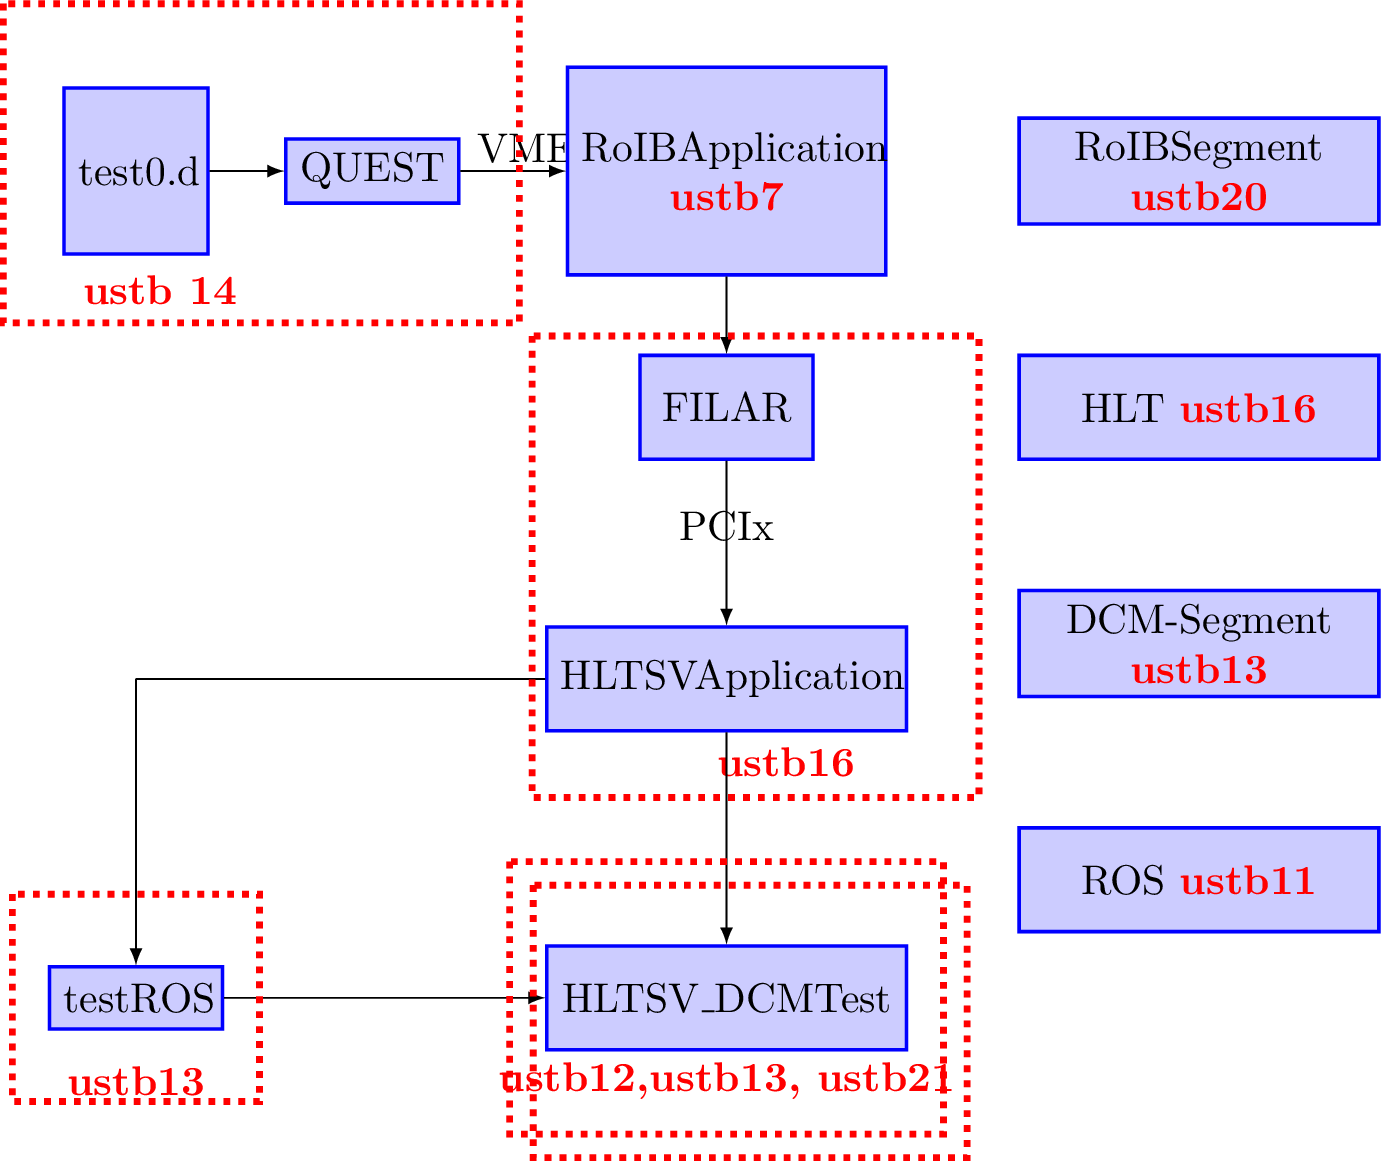
\includegraphics[width=0.8\linewidth]{figures/confOne.png}
\caption{A flow-chart showing {\bf Configuration 1} of the partition. This configuration was used to determine 
the optimal values of the parameters in Table~\ref{parameters} by producing the 
plots in Figures~\ref{para_plotsA}, \ref{para_plotsB} and \ref{para_plotsC}}.
\label{conf1}
\end{figure}

\begin{figure}[!h]
\centering
  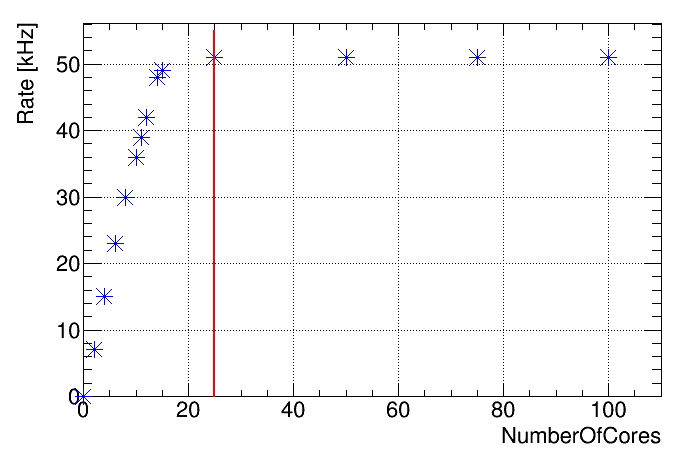
\includegraphics[width=0.8\textwidth]{figures/dcmVsRate.png}
	\caption{Plot showing the number of Cores maxes the rate at 25. The number of cores 
available on ustb13, ustb21 and ustb12 sums up to 20. An additional data point would show that 
the Number of Cores maxes at 20 }
  \label{para_plotsA}
\end{figure}

\begin{figure}[!h]
\centering
  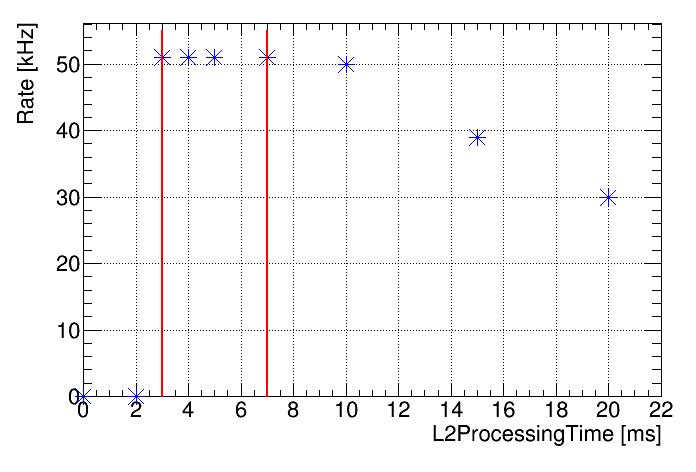
\includegraphics[width=0.8\textwidth]{figures/l2pVsRate.png}\\
	\caption{Plot showing the processing time less than 3\ ms is 
not physical. Above that, it makes sense that the rate would decrease 
}
  \label{para_plotsB}
\end{figure} 

\begin{figure}[!h]
\centering
  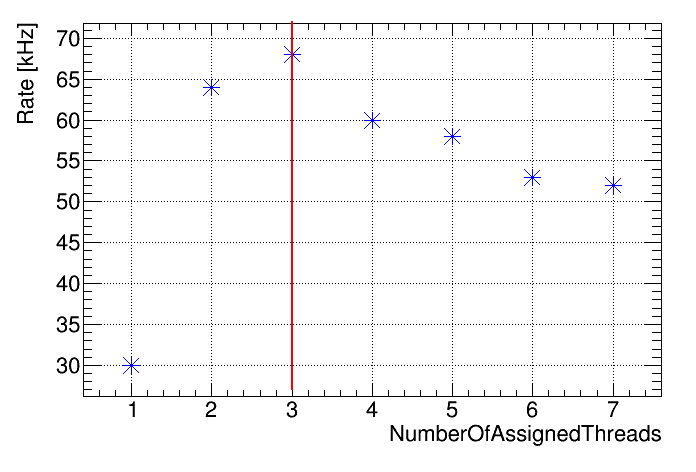
\includegraphics[width=0.8\textwidth]{figures/threads.png}
	\caption{Plot showing the number of threads assigned to the \acrshort{hltsv}}
  \label{para_plotsC}
\end{figure}

\par Using the plots in Figures~\ref{para_plotsA}\ref{para_plotsB}\ref{para_plotsC} it can be claimed that 
(25,5,3)\footnote{In this notation we put (NumberOfCores,L2ProcessingTime,NumberOfAssignedThreads)} 
is the optimal configuration; it was used as a starting point in the rest of the study. 
To test the CPU bottleneck, random data fragments were generated internally in 
the PC that hosts the \acrshort{hltsv} and by-passed the \acrshort{f} card. 
Data obtained through this method is referred to as {\it Internally Generated Data} (IGD).
Tests could therefore be conducted on powerful PCs that cannot host a \acrshort{f} card. The 
HLTSVApplication was put on ustb3 and ustb10 was used just for the \acrshort{dcm}s. The HLTSVApplication 
parameters were configured as (25,5,4). All other components of the partition remained identical to Configuration 1.
The schematic diagram on the left of Figures~\ref{conf2A} and \ref{conf2B} shows this setup.
In this configuration, the optimized rate was not expected to increase by running 
tdaq 05-03-00 (which has a default of \acrshort{f} 100 buffers) instead of tdaq 05-02-00 (1 buffer) 
because the \acrshort{roib} was by-passed. This achieved a rate of 68\ kHz. 
Adding another node to the \acrshort{dcm} (ustb4) boosted the rate to a stable 107\ kHz. The 
image on the right of Figure~\ref{conf2B} shows this new configuration, which is referred to here as 
{\bf Configuration 2}. Adding more than two \acrshort{dcm} nodes did not improve the rate. This implies that 
with at least two \acrshort{dcm}s a 100\ kHz rate is achievable on a powerful 
enough PC. Moving the HLTSVApplication to ustb16 (which has fewer number of cores and lower cache memory) 
gave an unstable rate ranging from 65\ kHz to 80\ kHz. The same behavior was observed in 
both tdaq 05-03-00 versions A and B\footnote{Reminder: The \acrshort{f} card in 
A has 100 buffers and in B has 16 buffers} as well.

\begin{figure}[!h]
\centering
  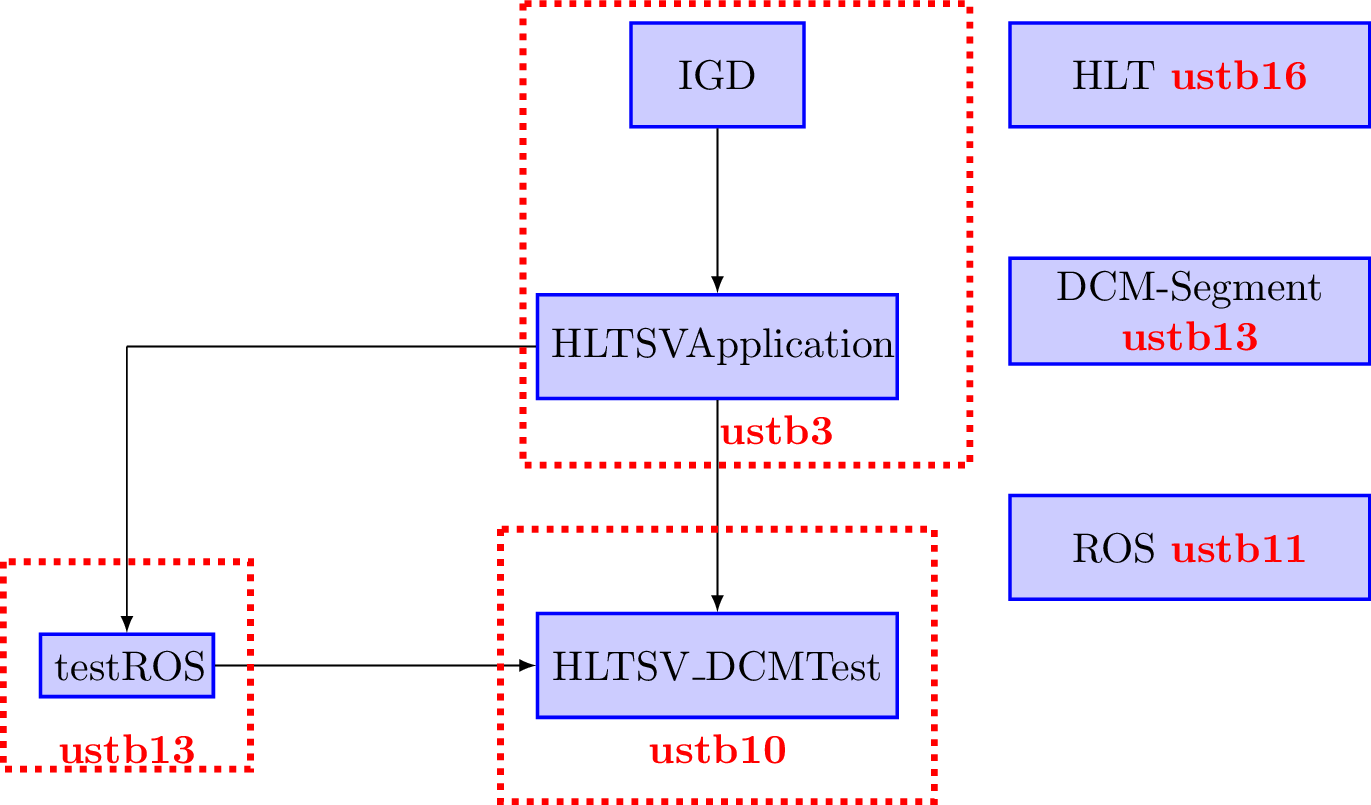
\includegraphics[width=0.8\textwidth]{figures/confTest.png}
  \caption{Flow chart showing configuration for running the partition without 
the \acrshort{roib}. The HLTSVApplication host generates random numbers in place of data. 
The HLTSVApplication was (25,5,4). The \acrshort{dcm}s and the HLTSVApplication were run 
on the test bed's most powerful PCs. 68\ kHz was achieved by this configuration} 
  \label{conf2A}
\end{figure}

\begin{figure}[!h]
\centering
  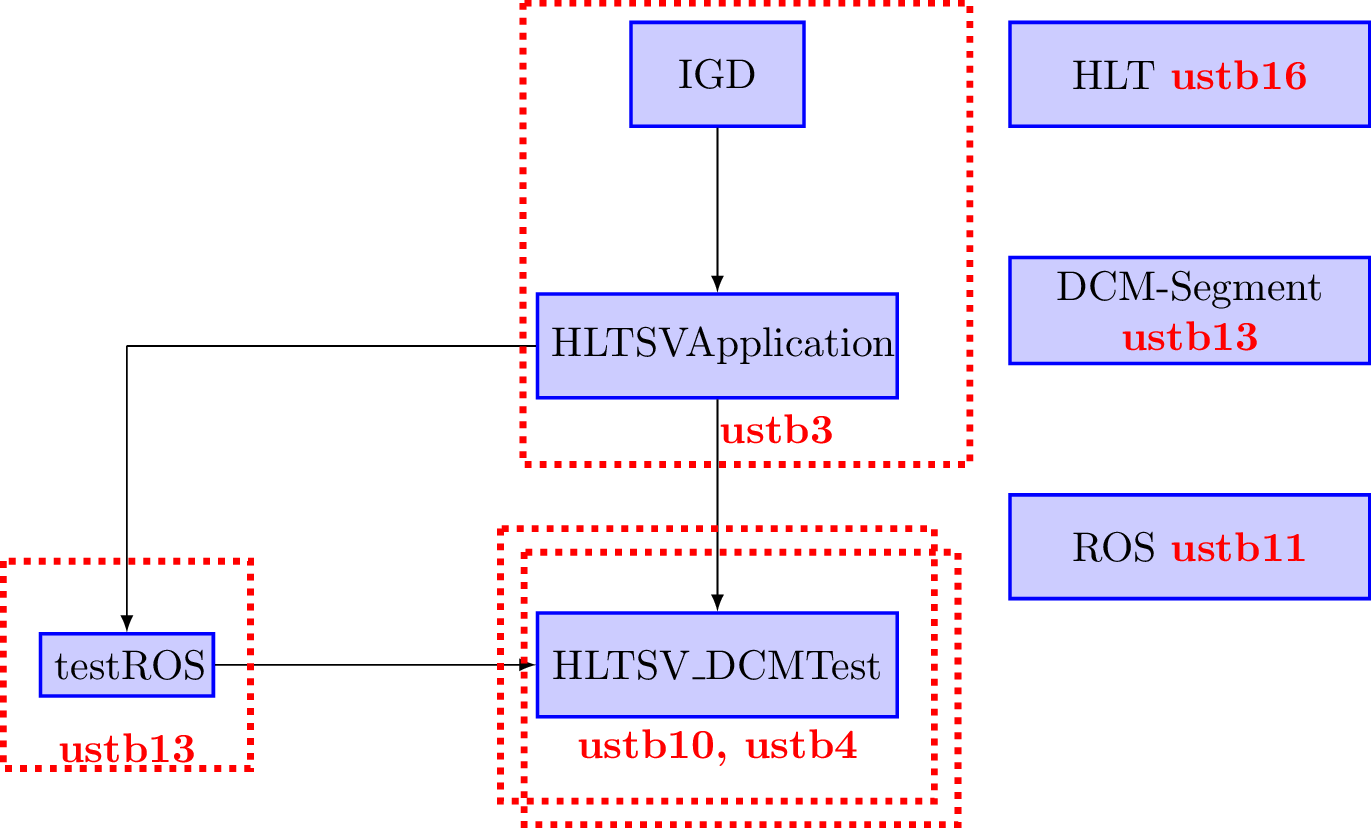
\includegraphics[width=0.8\textwidth]{figures/confTwo.png}
  \caption{Flow chart showing {\bf Configuration 2}. The only difference between this configuration and the one on 
the left is that there is an additional \acrshort{dcm} node (ustb4). The rate was boosted 
to 107\ kHz by adding this node. The \acrshort{hltsv} can therefore achieve 100\ kHz if it runs on a capable PC}
  \label{conf2B}
\end{figure}


\par To achieve a reproducible rate without the \acrshort{roib} with 
the HLTSVApplication on ustb16, NumberOfThreads were varied to find a value with 
a minimal rate fluctuation as shown in Figure~\ref{thr_again}. 
The error bars represent the rate fluctuation. Notice that at 7 threads, 
the rate stabilizes. HLTSVApplication configuration was then changed to (25,5,7). 
In addition to that, all segments (HLT, \acrshort{ros}, \acrshort{dcm}) were placed on ustb21. The 
HLTSV\_DCM application ran on ustb10 and ustb4. The partition was hosted by ustb13. The 
image in Figure~\ref{confTwoABCa} shows a schematic of a version of 
Configuration 2 but with the above changes; the rate still stabilized at 107\ kHz.  
This configuration is referred to as {\bf Configuration 2a}.  With the HLTSVApplication on ustb16,({\bf Configuration 2b}, 
Figure~\ref{confTwoABCb}) the rate stabilizes at 85\ kHz. Because ustb16 has 
fewer cores and lower cache memory than ustb3, this implies that the rate decreases because of the 
CPU bottleneck. To eliminate the possibility that this decrease in rate is dependent on the PC 
architecture\footnote{ustb16 is 32-bit whereas ustb3 is 64-bit} the HLTSVApplication was moved to 
ustb12,({\bf Configuration 2c}, Figure~\ref{confTwoABCc}) which has identical memory 
to ustb16 but is 64-bit; the rate was 85\ kHz as well. 

\begin{figure}[!h]
\centering
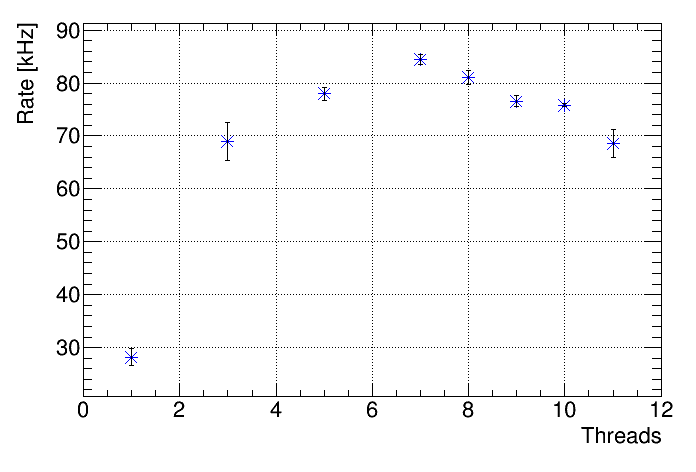
\includegraphics[width=0.8\linewidth]{figures/threads_presFive.png}
\caption{Plot showing rate variation with the number of threads. At 7 number of threads the rate is highest and the most stable. The error bars show the instability}
\label{thr_again}
\end{figure}


\begin{figure}
\centering
\begin{subfigure}{0.4\textwidth}
  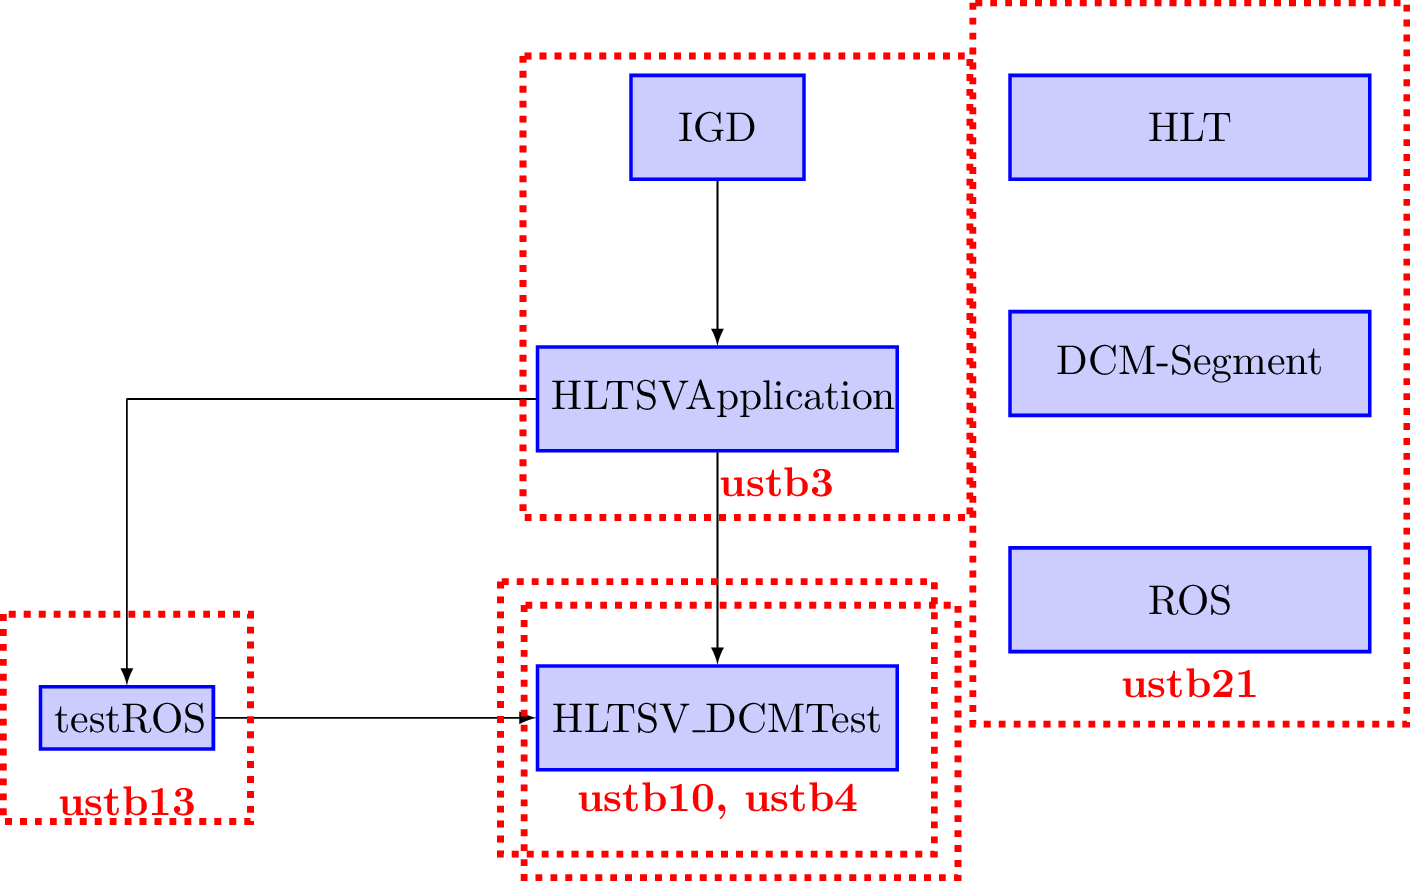
\includegraphics[width=\textwidth]{figures/confTwoA.png}
  \caption{Configuration 2a: When the HLTSVApplication is on ustb3, 
the rate maxes at 107\ kHz. ustb3 is 64-bit. Here its configuration is (25,5,7). This rate 
ensures a stable ratewhen the \acrshort{roib} is added}
  \label{confTwoABCa}
\end{subfigure}\hspace{0.1\textwidth} %
\begin{subfigure}{0.4\textwidth}
  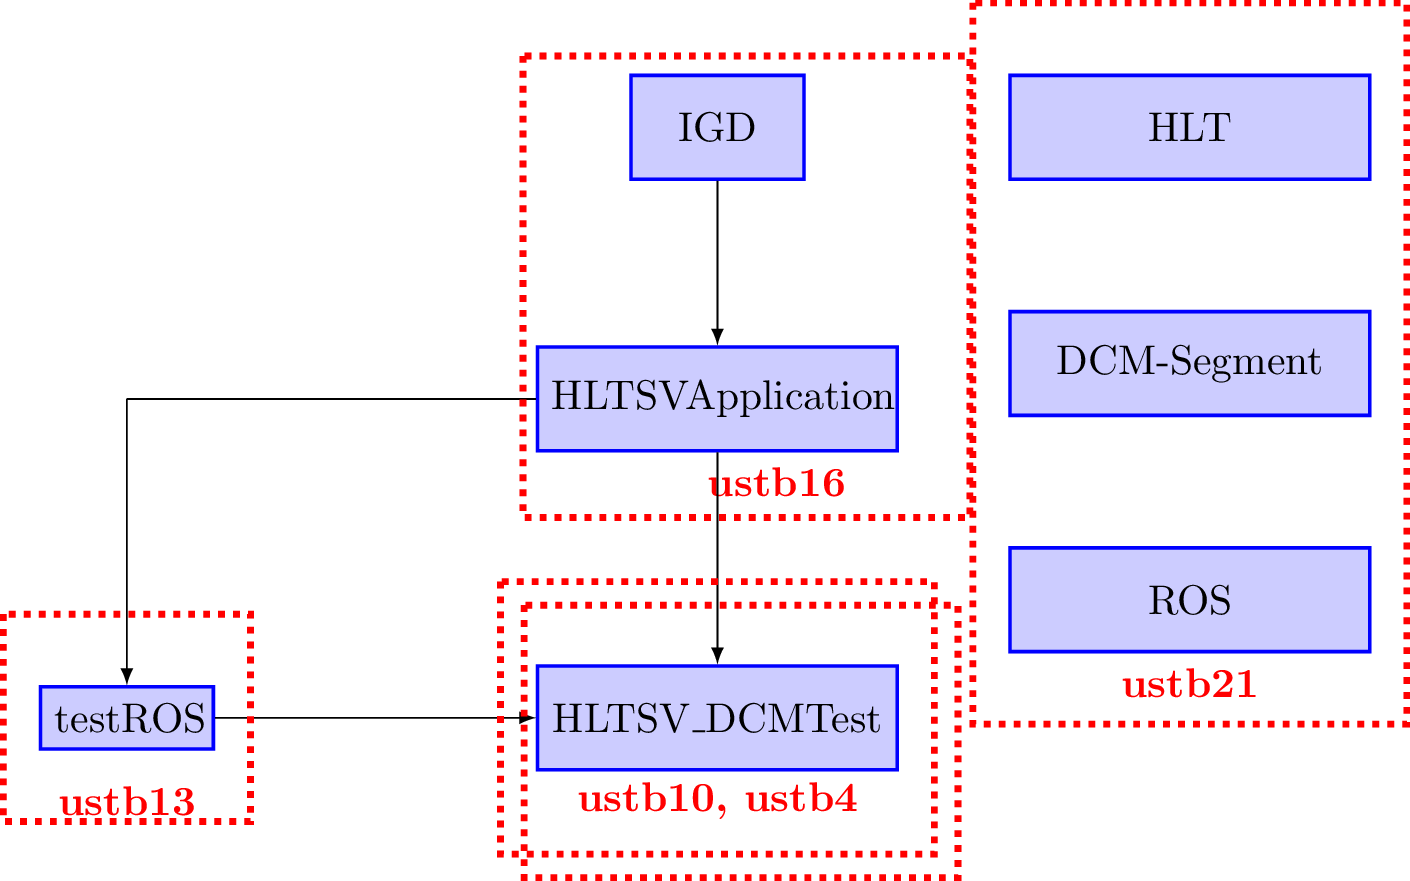
\includegraphics[width=\textwidth]{figures/confTwoB.png}
  \caption{Configuration 2b: Moving the HLTSVApplication to ustb16 decreases the rate to 85\ kHz. ustb16 
is 32-bit and has lower number of cores than ustb3}
  \label{confTwoABCb}
\end{subfigure}\\[1ex]
\begin{subfigure}{0.4\textwidth}
  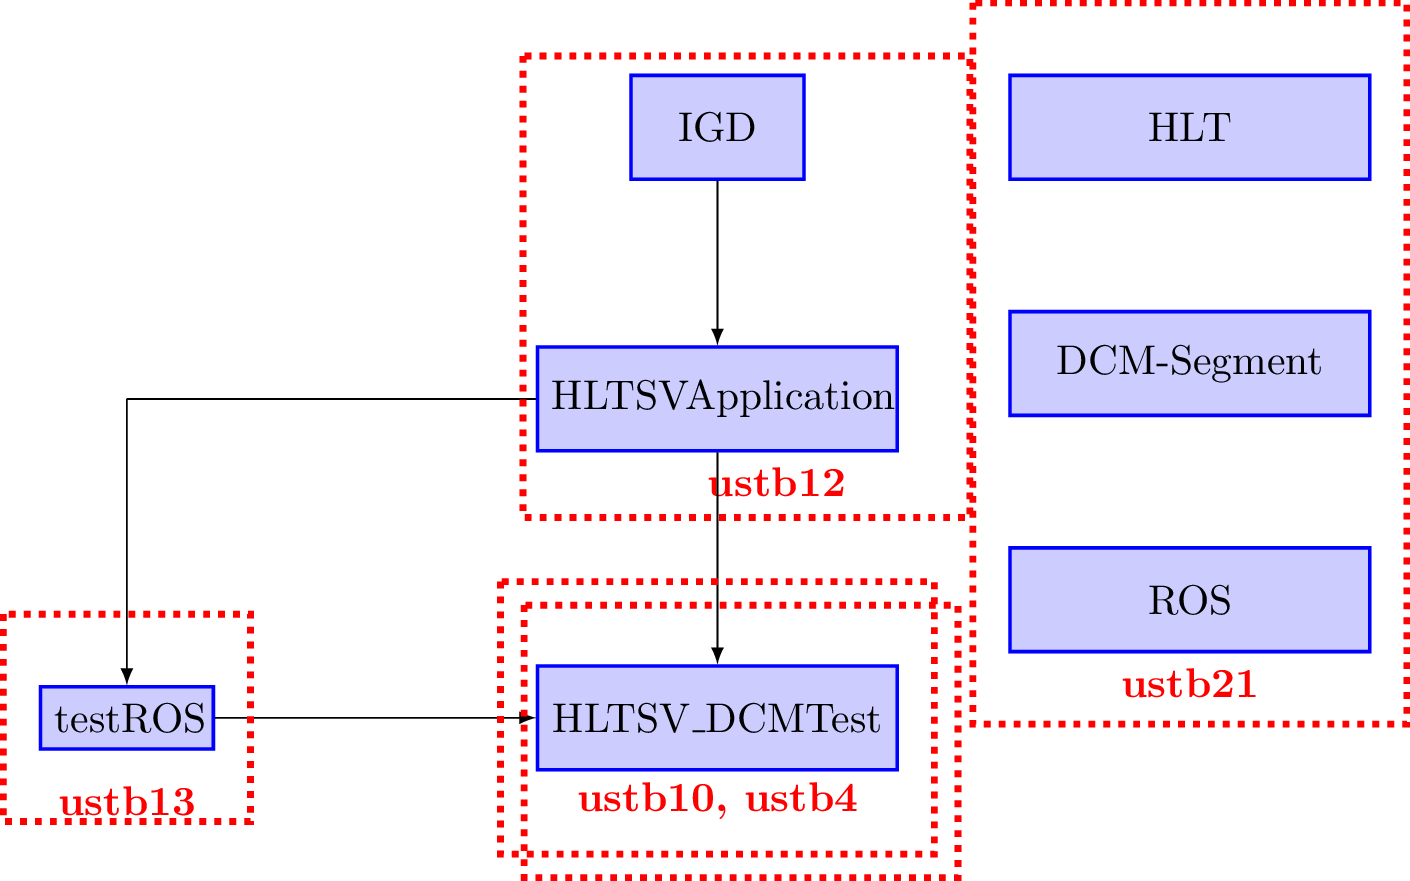
\includegraphics[width=\textwidth]{figures/confTwoC.png}
  \caption{Configuration 2c: Moving the HLTSVApplication to ustb12 achieves 85\ kHz maximum as well. ustb12 
is 64-bit but has less memory than ustb3. The rates quoted here are 
from tdaq 05-02-00 (see Table~\ref{sumry}.) \acrshort{hltsv} rate measurements are 
hampered by CPU memory and number of cores}
  \label{confTwoABCc}
\end{subfigure}
\caption{Illustrations of 3 variations of Configuration 2}
\end{figure}

\par Adding a 1-input \acrshort{roib} to this system lowered the \acrshort{hltsv} rate 
even further to 55\ kHz. Tests were performed with two and three \acrshort{roib} inputs
 as well, referred to as {\bf Configuration 3} and shown in Figure~\ref{confThree}. 
In this configuration the RoIBSegment was added to ustb21 as well. The rate successively fell with increasing 
inputs as expected. The third column in Table~\ref{sumry} summarizes these rates. The CPU bottleneck 
therefore does not permit measurement of the rate of fragment transfer 
between the \acrshort{roib} and the \acrshort{hltsv}.  

\begin{figure}[!h]
\centering
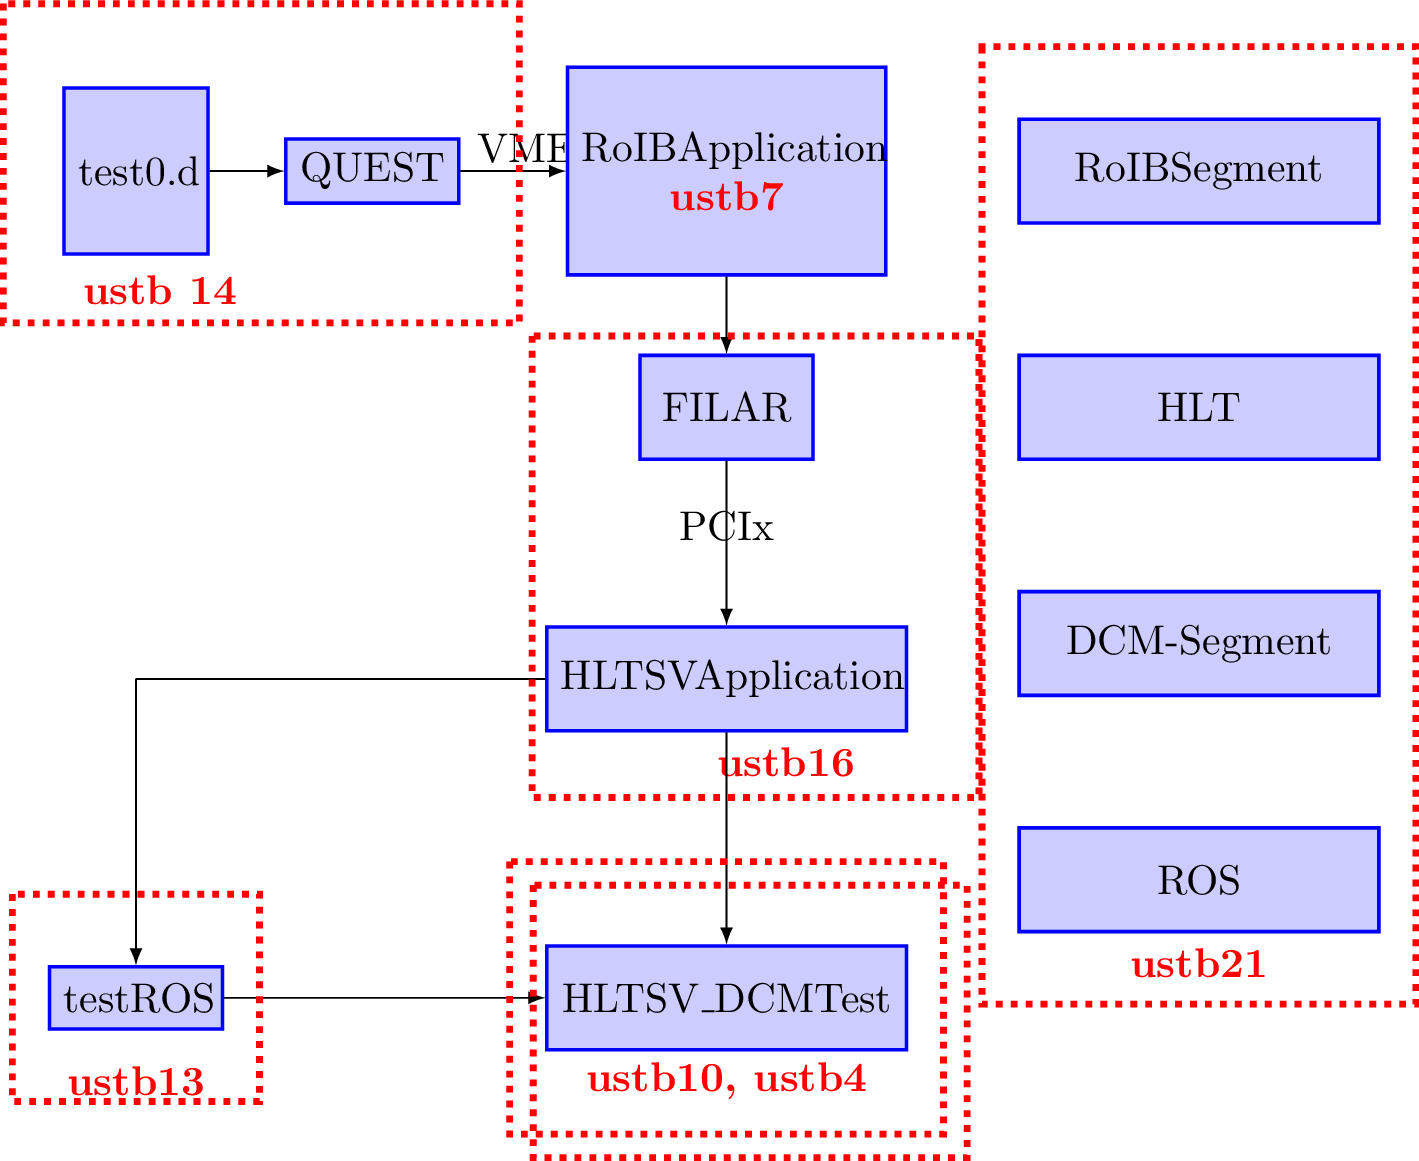
\includegraphics[width=0.7\linewidth]{figures/conf3.png}
\caption{Configuration 3: The \acrshort{roib} is added and real data fragments are 
read. The rate maxes at 55\ kHz with 1 \acrshort{roib} input (see Table~\ref{sumry}) }
\label{confThree}
\end{figure}

\par Tdaq 05-03-00 was expected to improve the rates when running partitions with 
the \acrshort{roib}. Rate changes were not expected for those partitions that do not 
include the \acrshort{roib}. This is because the main difference between tdaq 05-02-00 
and tdaq 05-03-00 is the \acrshort{f} buffer size. Partitions with no \acrshort{roib} do not 
use the \acrshort{f} card so no improvement was expected. For Configurations 2a and 2b the rates were 
identical to the tdaq 05-02-00 for both version A and B of tdaq 05-03-00. 
Configuration 2c in both versions A and B produced largely varying rates ranging between 
56\ kHz and 93\ kHz. The average rate over 12 data points for A and B was 81\ kHz and 
82.5\ kHz respectively for Configuration 3 (See Table~\ref{sumry}). These large 
variations were observed only when the HLTSVApplication was on 32-bit PCs.  
 
\par For Configuration 3 varying rates were observed in both A and B 
versions of tdaq 05-03-00. Figure~\ref{avs} shows the rates recorded for these two 
versions with the \acrshort{roib} included. The rates recorded in 
Table~\ref{sumry} are averages over the data points in Figure~\ref{avs}. Although 
there is a significant increase in rates from tdaq 05-02-00 to tdaq 05-03-00, due 
to the instabilities and few data points it is impossible to categorically identify an increase in rate from A to B.

\begin{table}[!h]
\begin{center}
\begin{tabular}{c|c|c|c|c}
& Configuration& tdaq 05-02-00 & tdaq 05-03-00 & tdaq 05-03-00 \\
&  & [kHz]         &  A [kHz]    & B [kHz] \\
\hline\hline
\multirow{3}{*}{Without \acrshort{roib}}& 2a & 107 & 107 & 107 \\ 
& 2b & 85 & 85  & 85 \\ 
& 2c & 85 & 81 (v) & 82.5 (v) \\ 
\hline
\multirow{3}{*}{With \acrshort{roib}} & 3 (1 input)   & 55 & 76 (v) & 73 (v) \\
& 3 (2 input)   & 49 & 62 (v) & 74 (v) \\ 
& 3 (3 input)   & 44 & 59 (v) & 62 (v)
\end{tabular}
\end{center}
\caption{Summary of \acrshort{hltsv} rates for all tested configurations in all 
releases of the tdaq software. The {\it v} next to a rate indicates that the rate 
recorded is an average over multiple rates because of the large rate variations. Version A 
and B of software differ over the number of buffers available to the \acrshort{f} card; 100 
for A and 16 for B. For tdaq 05-02-00 the buffer size is 1. There is a general increase in the 
rate from tdaq 05-02-00 to tdaq 05-03-00.}
\label{sumry}
\end{table}

\par To rule out the possibility of the instabilities stemming from the \acrshort{f} card, 
tests similar to Configuration 3 were performed using the \acrshort{t} card. Instead of 
replacing the FIILAR with the \acrshort{t} on ustb16, the \acrshort{t}  and 
the \acrshort{f} cards were installed on ustb11; it was therefore necessary to run the HLTSVApplication on ustb11. 
Table~\ref{tilar} and Table~\ref{filar11} show the rates for these tests. The instabilities 
still existed. Again, for unstable rates the entries are just averages over a few data 
points so it was not possible to tell if there is an improvement from version A to version B of 
tdaq 05-03-00. There seemed to be an improvement however from tdaq 05-02-00 to tdaq 05-03-00. 
Also, higher rates were generally observed when the FILAR card. 

\begin{table}[!h]
\begin{center}
\begin{tabular}{c|c|c|c}
 Number of   & tdaq 05-02-00 & tdaq 05-03-00 & tdaq 05-03-00 \\
 \acrshort{roib} Inputs & [kHz]         &  A [kHz]    & B [kHz] \\
\hline\hline
 1    & 43 & 60 (v) & 57 (v) \\
 2    & 40 & 54 (v) & 54 (v) \\ 
 3    & 36 & 49 (v) & 54 (v)
\end{tabular}
\end{center}
\caption{Summary of \acrshort{hltsv} rates with the \acrshort{roib} in all releases 
of the tdaq software using the \acrshort{t} card. The configuration is similar to 
Configuration 3, but with HLTSVApplication running on ustb11. The large variations in 
rates were still observed so there was nothing wrong with the \acrshort{f} card.}
\label{tilar}
\end{table}

\begin{table}[!h]
\begin{center}
\begin{tabular}{c|c}
 Number of    & tdaq 05-03-00 \\
 \acrshort{roib} Inputs  & B [kHz] \\
\hline\hline
 1     & 70 (v) \\
 2     & 63 (v) \\ 
 3     & 55 (v)
\end{tabular}
\end{center}
\caption{Summary of \acrshort{hltsv} rates with the \acrshort{roib} in version B of 
tdaq 05-03-00 using the \acrshort{f} card. The configuration is similar to Configuration 3, 
but with HLTSVApplication running on ustb11. The average rates observed 
are larger than those observed with a TILAR card as shown in Table~\ref{tilar}.}
\label{filar11}
\end{table}

\begin{figure}[!h]
  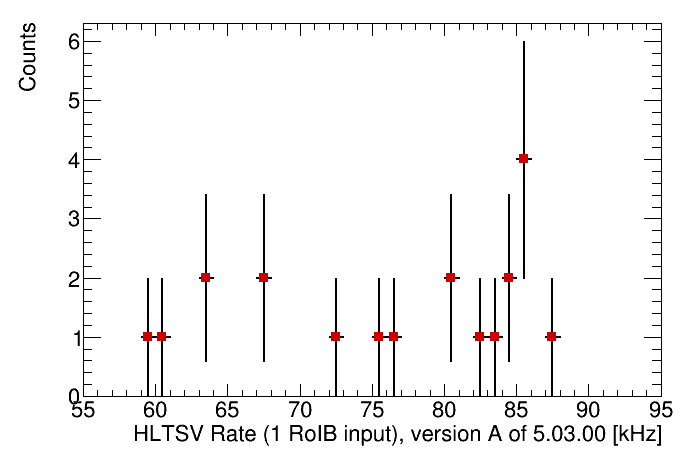
\includegraphics[width=0.49\textwidth]{figures/h_jim_roib.png}
  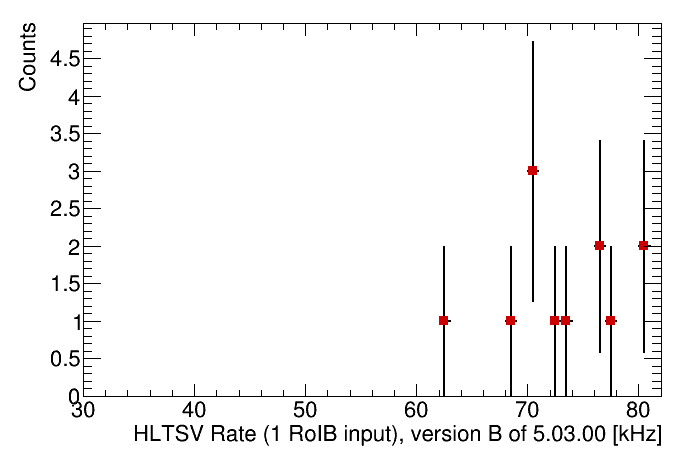
\includegraphics[width=0.49\textwidth]{figures/h_reinerOne.png}\\
  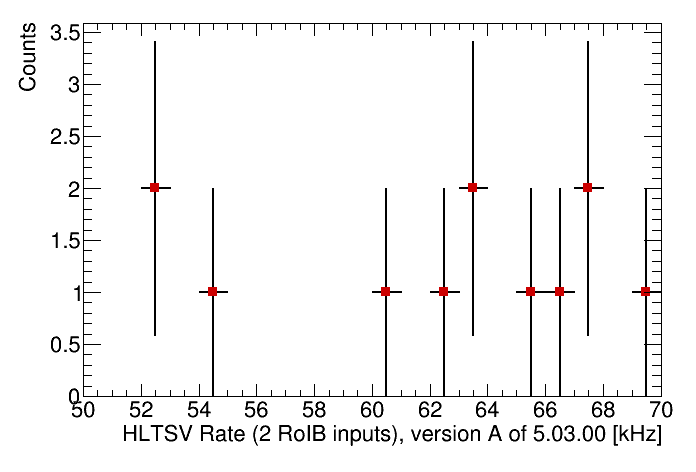
\includegraphics[width=0.49\textwidth]{figures/h_jimTwo.png}
  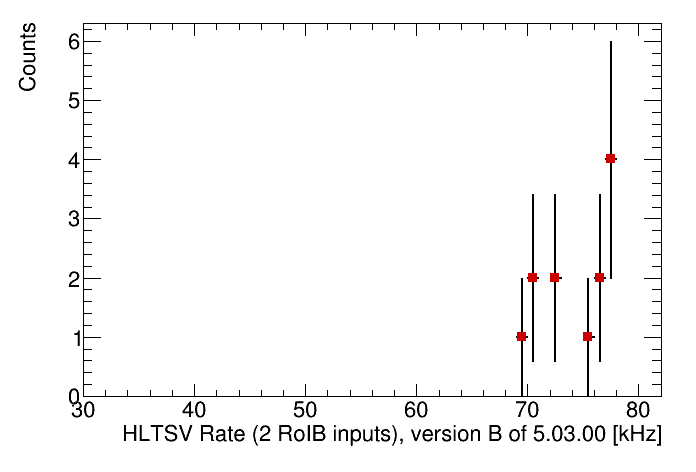
\includegraphics[width=0.49\textwidth]{figures/h_reinerTwo.png}\\
  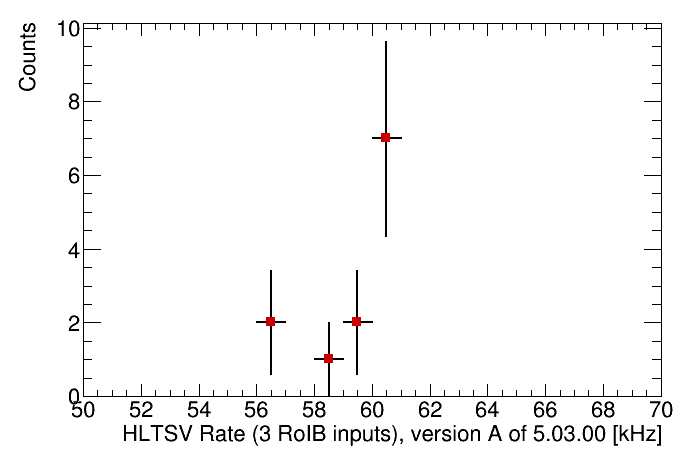
\includegraphics[width=0.49\textwidth]{figures/h_jimThree.png}
  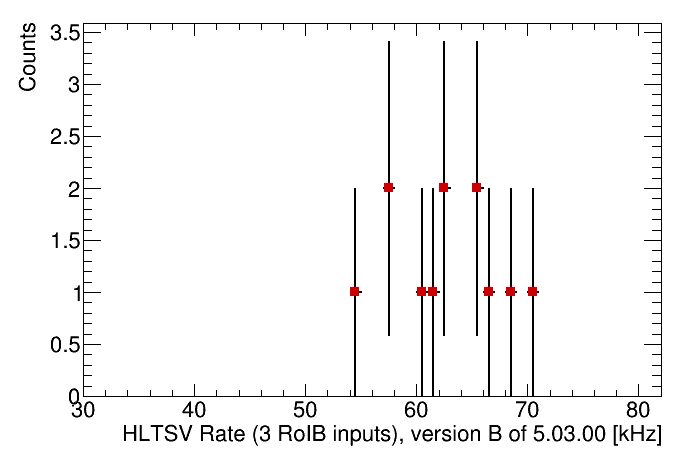
\includegraphics[width=0.49\textwidth]{figures/h_reinerThree.png}\\
  \caption{Plots showing rate variations under several configurations.
Each plot shows rates recorded independently but under Configuration 3. 
Differences between versions A and B are extensively discussed in the text. These 
large variations are still not understood, but they are only observed when 
the HTSVApplication is running of 32-bit PCs. Their averages are entered in Table~\ref{sumry}}
  \label{avs}
\end{figure}
